\documentclass[tikz, dvisvgm, border=5mm]{standalone}
\usetikzlibrary{calc, angles, quotes}

\begin{document}
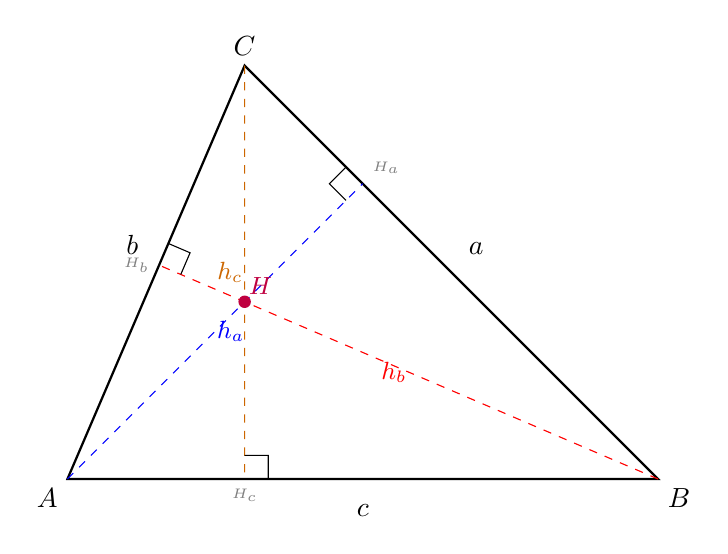
\begin{tikzpicture}[scale=1.5]

    % 1. Definition der Eckpunkte (Allgemeines/schiefwinkliges Dreieck)
    \coordinate (A) at (0,0);
    \coordinate (B) at (5,0);
    \coordinate (C) at (1.5,3.5);

    % 2. Zeichnen des Dreiecks
    \draw[thick] (A) -- (B) -- (C) -- cycle;

    % 3. Automatische Berechnung der Höhenfußpunkte (Projektion)
    \coordinate (Ha) at ($(B)!(A)!(C)$); % Projektion von A auf BC
    \coordinate (Hb) at ($(A)!(B)!(C)$); % Projektion von B auf AC
    \coordinate (Hc) at ($(A)!(C)!(B)$); % Projektion von C auf AB

    % 4. Berechnung des Höhenschnittpunkts (Schnittpunkt zweier Höhen)
    \coordinate (H) at (intersection of A--Ha and B--Hb);

    % 5. Zeichnen der Höhen (gestrichelt und farbig für bessere Übersicht)
    \draw[blue, dashed] (A) -- (Ha) node[midway, right=-1mm, font=\small] {$h_a$};
    \draw[red, dashed] (B) -- (Hb) node[midway, left=-1mm, font=\small] {$h_b$};
    \draw[orange!80!black, dashed] (C) -- (Hc) node[midway, left=-1mm, font=\small] {$h_c$};

    % 6. Rechte Winkel einzeichnen
    \pic [draw, angle radius=3mm] {right angle = A--Ha--C};
    \pic [draw, angle radius=3mm] {right angle = B--Hb--C};
    \pic [draw, angle radius=3mm] {right angle = C--Hc--B};

    % 7. Punkte markieren (Höhenschnittpunkt)
    \fill[purple] (H) circle (1.5pt) node[shift={(0.2,0.2)}, font=\small] {$H$};

    % 8. Beschriftung der Ecken und Seiten
    % Ecken
    \node[below left] at (A) {$A$};
    \node[below right] at (B) {$B$};
    \node[above] at (C) {$C$};
    
    % Höhenfußpunkte
    \node[above right, font=\tiny, text=gray] at (Ha) {$H_a$};
    \node[left, font=\tiny, text=gray] at (Hb) {$H_b$};
    \node[below, font=\tiny, text=gray] at (Hc) {$H_c$};

    % Seiten (mittig platziert mit leichtem Versatz nach außen)
    \path (A) -- (B) node[midway, below=2mm] {$c$};
    \path (B) -- (C) node[midway, above right=1mm] {$a$};
    \path (C) -- (A) node[midway, above left=1mm] {$b$};

\end{tikzpicture}
\end{document}
